\documentclass[a4paper]{article}

\usepackage[english]{babel}
\usepackage[utf8x]{inputenc}
\usepackage{amsmath}
\usepackage{amsfonts}
\usepackage{graphicx}
\usepackage[]{algorithm2e}
\usepackage[colorinlistoftodos]{todonotes}

\title{CS 5785 -- Applied Machine Learning -- Lec.\ 12}
\author{Prof.\ Nathan Kallus, \\Scribe: TBD}
\date{Oct.\ 12, 2017}

\begin{document}
\maketitle


\section{Clustering}

\subsection{Review from Last Time}
$K$-means is an iterative clustering algorithm that divides a set of feature vectors into $K$ clusters.  One caveat of using $K$-means is that it assumes our data lives in a vector space and that we can compute Euclidean distance between these data points.  In practice, not all clustering problems come to us with this representation.
\subsection{Definitions}
A clustering algorithm is an unsupervised method that finds a cluster $C$ such that $C:\{1, ..., N\} \rightarrow \{1, ..., k\}$ in order to minimize the with-in cluster variance.

Multi-dimensional scaling methods use a distance Matrix $D \in R^{N\times N}$ to find vectors $x_1, ..., x_n \in R^N$ such that $||x_i - x_j||_2 \approx D_{ij}$
\subsection{K-Medoids}

\begin{figure}
\centering
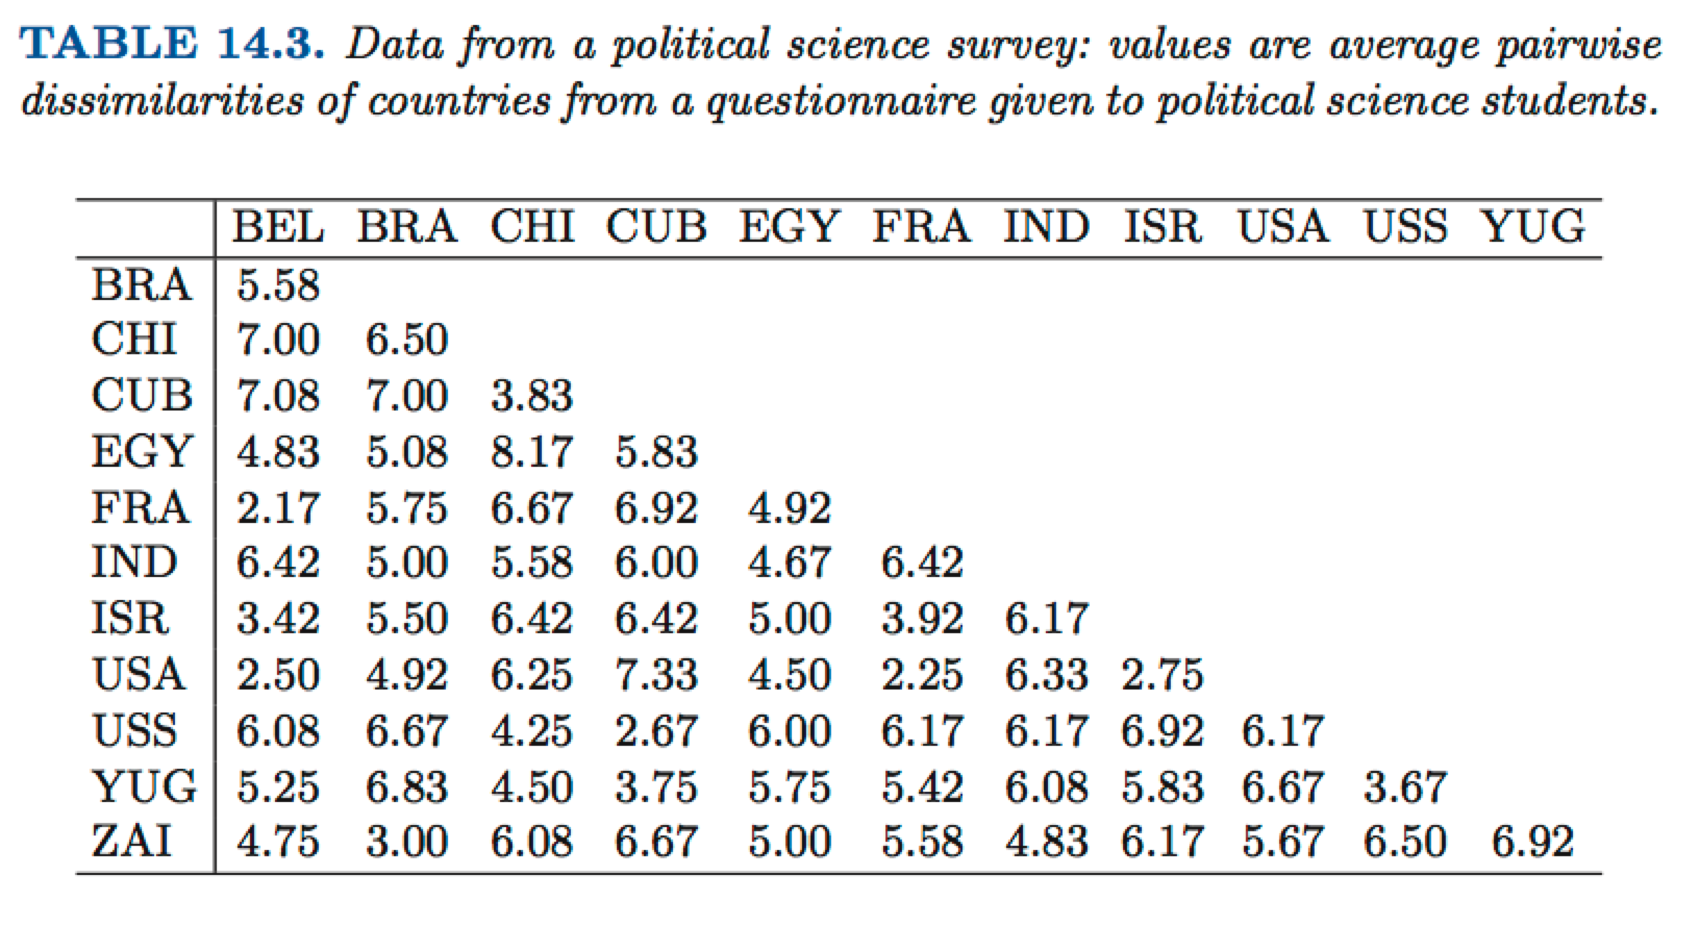
\includegraphics[width=1.0\textwidth]{DissimilaritiesTable.png}
\caption{\label{fig:dissimilaritiesTable} The missing data is symmetric to the existing data}
\end{figure}

In cases where we have a table of dissimilarities without access to the vector space from which they arose, as seen in Figure \ref{fig:dissimilaritiesTable}, we can't use $K$-Means, but we can use $K$-Medoids instead. $K$-Medoids restricts the cluster centers to lie on existing data points (as opposed to $K$-Means that uses vector averages) but other than that it is very similar to $K$-means, see Algorithm \ref{alg:KMedoids}. $K$-Medoids is a central clustering method, as opposed to $K$-means, which is a pairwise clustering method.

\begin{algorithm}
 \KwData{Dissimilarities table D, $K$}
 \KwResult{$K$ clusters}
 initialize $C$\;
 \While{$C$ changes}{
  \begin{itemize}
  \item Find the medoid for each cluster:\\
  $$i_k^*=\underset{\{i:C(i)=k\}}{\arg\min} \sum_{C(i')=k} D(x_i, x_i')$$\\
  \item Set $m_k=x_{i_k^*}$ for $k = 1, 2, \ldots , K$. \\
  \item Assign each observation to the closest medoid:\\
  $$C(i)=\underset{1 \leq k \leq K}{\arg\min} \quad D(x_i, m_k)$$
  \end{itemize}
 }
 \caption{$K$-Medoids [HTF Algorithm 14.2]}
 \label{alg:KMedoids}
\end{algorithm}

Later in the course we'll learn about another unsupervised learning method called \emph{Multidimensional Scaling} (MDS) that also operates on dissimilarity matrices.  Whereas $K$-Medoids simply aims to cluster the data, MDS seeks a low dimensional vector embedding that fits the observed dissimilarities.

Like K-Means clusteing, K-Medoids clustering has an objective function given by 
$$w'(c) = \sum_{k=1}^{K}\sum_{C(i) = k} D_{ii_{k}}^*$$

Note that because the objective function decreases in each iteration step and because there is a finite number of elements in the dataset, the K-Medoids algorithm will terminate in finite time.
\subsection{Hierarchical Clustering}
$K$-medoids, like $K$-means, requires us to choose $K$, which as we've seen before can be tricky.  One way around this problem is to use an \emph{agglomerative} (bottom up) or \emph{divisive} (top down) method, which result in a hierarchical clustering. Agglomerative clustering works as follows:
\begin{enumerate}
\item Initialization: Start with every data point as a singleton cluster ($|C|=N$).
\item Step: Merge the closest two clusters ($|C_{new}| = |C_{old}| + 1$).
\item Repeat 1 and 2 until everything is merged ($|C| = 1$).
\item Return the list of merges preformed in the correct order (See Figure \ref{fig:Hierarchy}).
\end{enumerate}

\begin{figure}
\centering
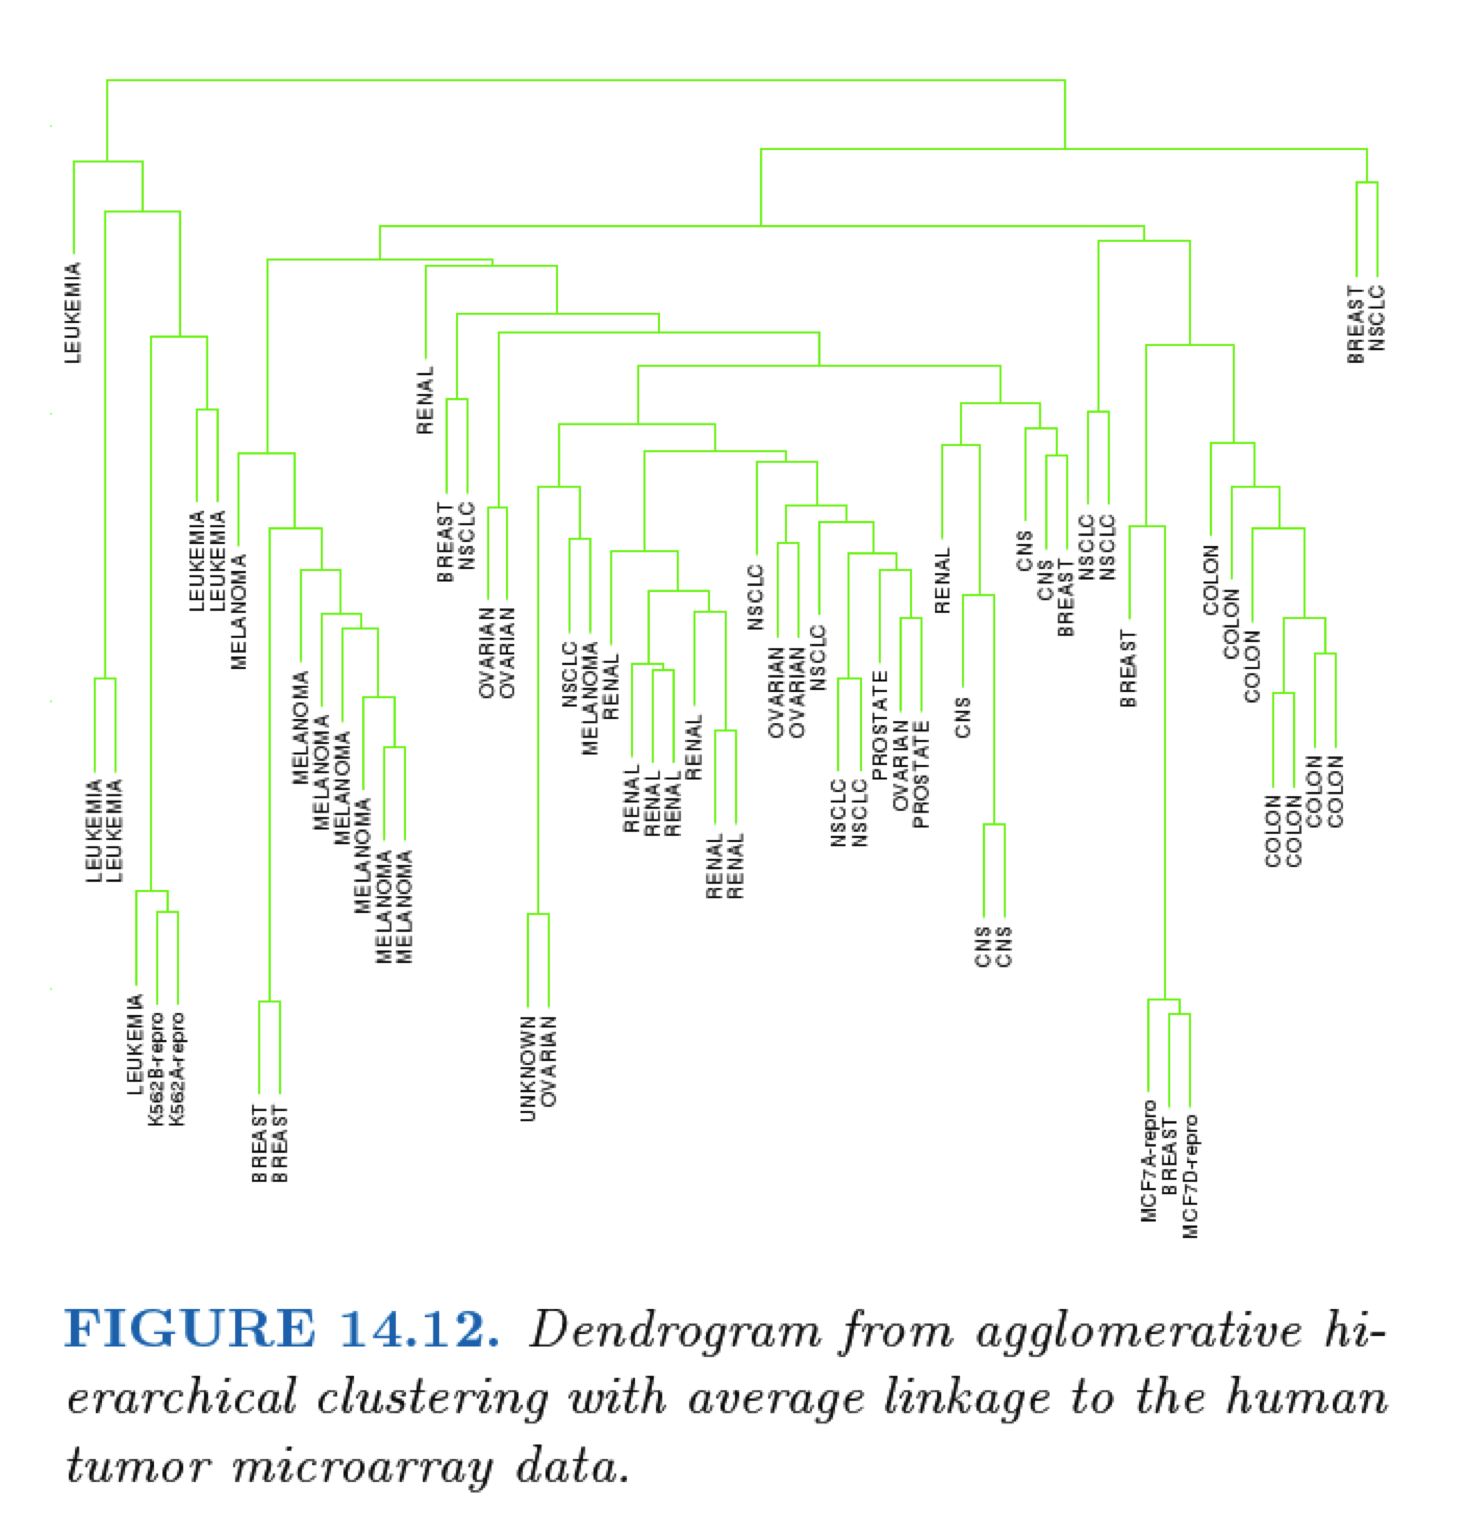
\includegraphics[width=1.0\textwidth]{HierarchicalClustering.png}
\caption{\label{fig:Hierarchy} The return value of the \textit{Hierarchical Clustering} algorithm}
\end{figure}

There are a number of ways to measure dissimilarities between two groups of data points resulting from the merging steps:
\begin{enumerate}
\item Single Linkage - The distance between the groups is the distance between the closest pair of data points, one from each group: $$d_{SL}(G,H)=\min_{\substack{
   i \in G \\
   i' \in H
  }} d_{ii'}$$
\item Complete Linkage - The distance between the groups is the distance between the farthest pair of data points, one from each group: $$d_{CL}(G,H)=\max_{\substack{
   i \in G \\
   i' \in H
  }} d_{ii'}$$
\item Group Average - The distance between the groups is the average distance between each pair of data points, one from each group: $$d_{GA}(G,H)=\frac{1}{N_G N_H}\;\sum_{i \in G}\;\sum_{i' \in H} d_{ii'}$$
\end{enumerate}

\begin{figure}
\centering
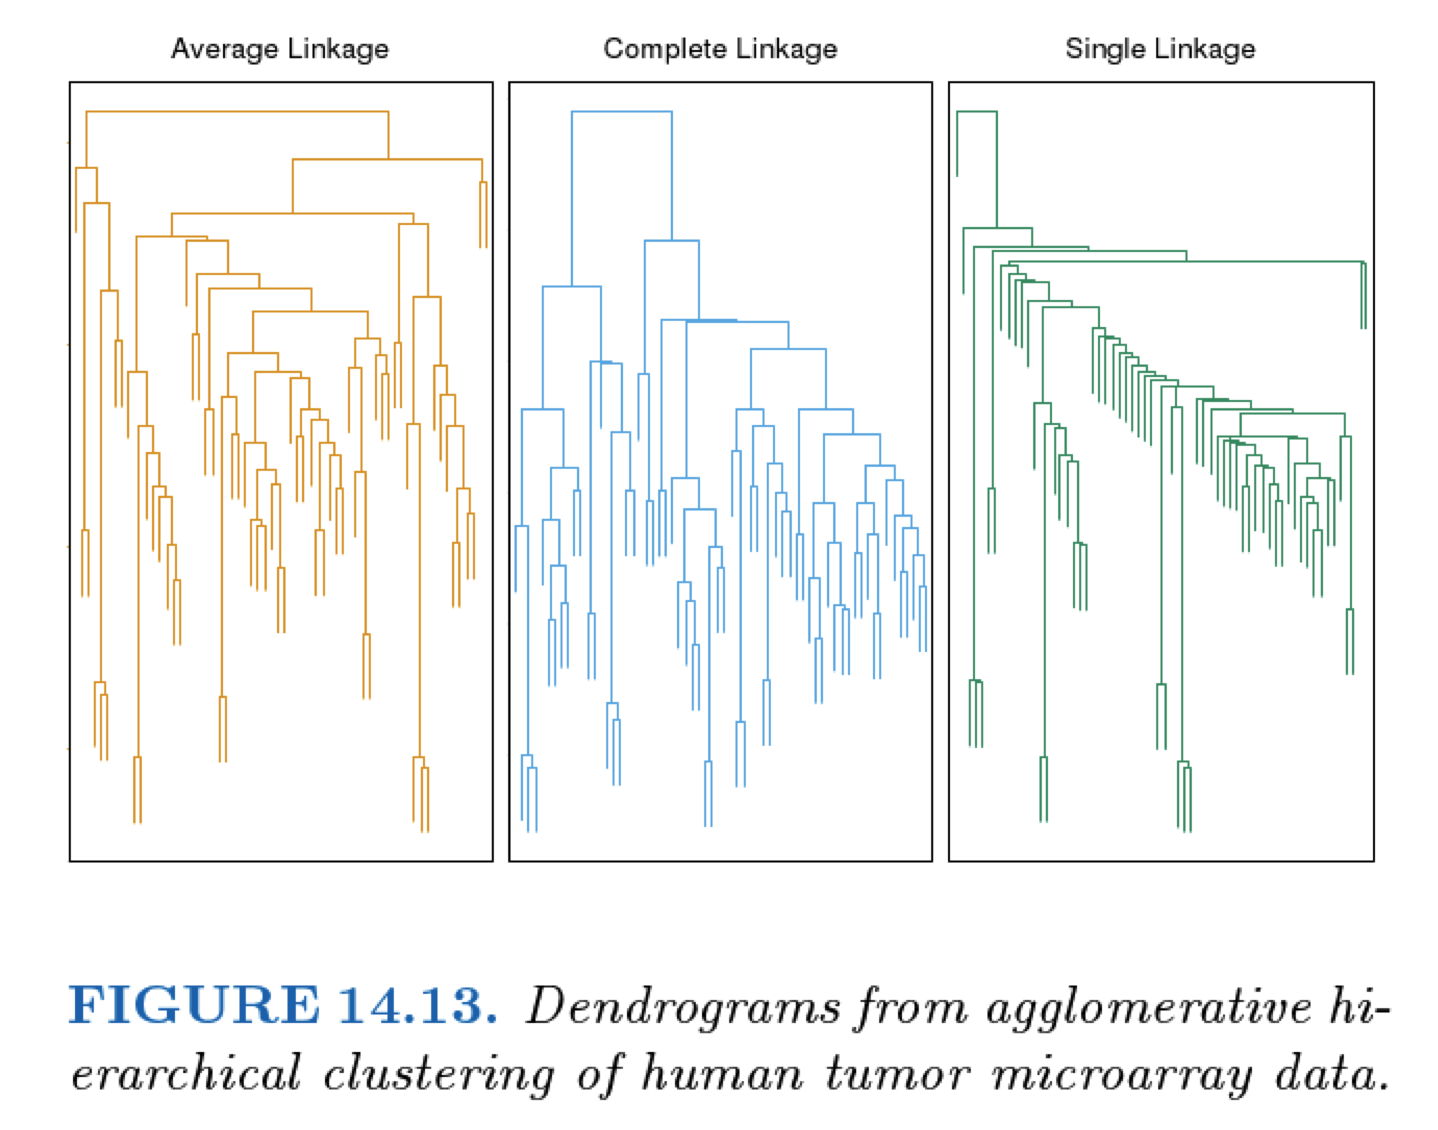
\includegraphics[width=1.0\textwidth]{HierarchicalPhases.png}
\caption{\label{fig:MergingTechniques} The output of the hierarchical clustering algorithm when using different merging techniques.}
\end{figure}

See Figure \ref{fig:MergingTechniques} for the difference in the results of the algorithm when using the different merging techniques. Similarly, divisive clustering starts with all data points in one merged cluster and iterates until each data point is in its own singleton cluster. 

If we want to return a partitioning of the original dataset to clusters we choose a level in the returned hierarchy and return the partitioning up to that level. We can imagine a dial that we can turn to move up and down in the levels of the hierarchy and see the clusters change, enabling us to choose the level most appropriate to our use case. 

\section{Principal Components Analysis (PCA)}
PCA is an unsupervised dimensionality reduction technique used to find axes of variations in a dataset.  In a sense, clustering may also be viewed as an unsupervised dimensionality reduction technique, in that it assigns possibly high dimensional feature vectors to one of $K$ tokens (cluster labels). Clustering is useful when the data is \textit{clumpy}, e.g., arranged in a manner reminiscent of Gaussian point clouds. For example, if a group of people play darts on a single target the darts would be arranged in a clump around the bullseye. Clumpy data is well represented by tokens or cluster centers. PCA is useful for ``manifoldy'' data (specifically, linear manifolds), which is well represented in low dimension coordinate system.  Often, problems that are well suited to $K$-means are ill suited to PCA and vice versa.

\begin{figure}
\centering
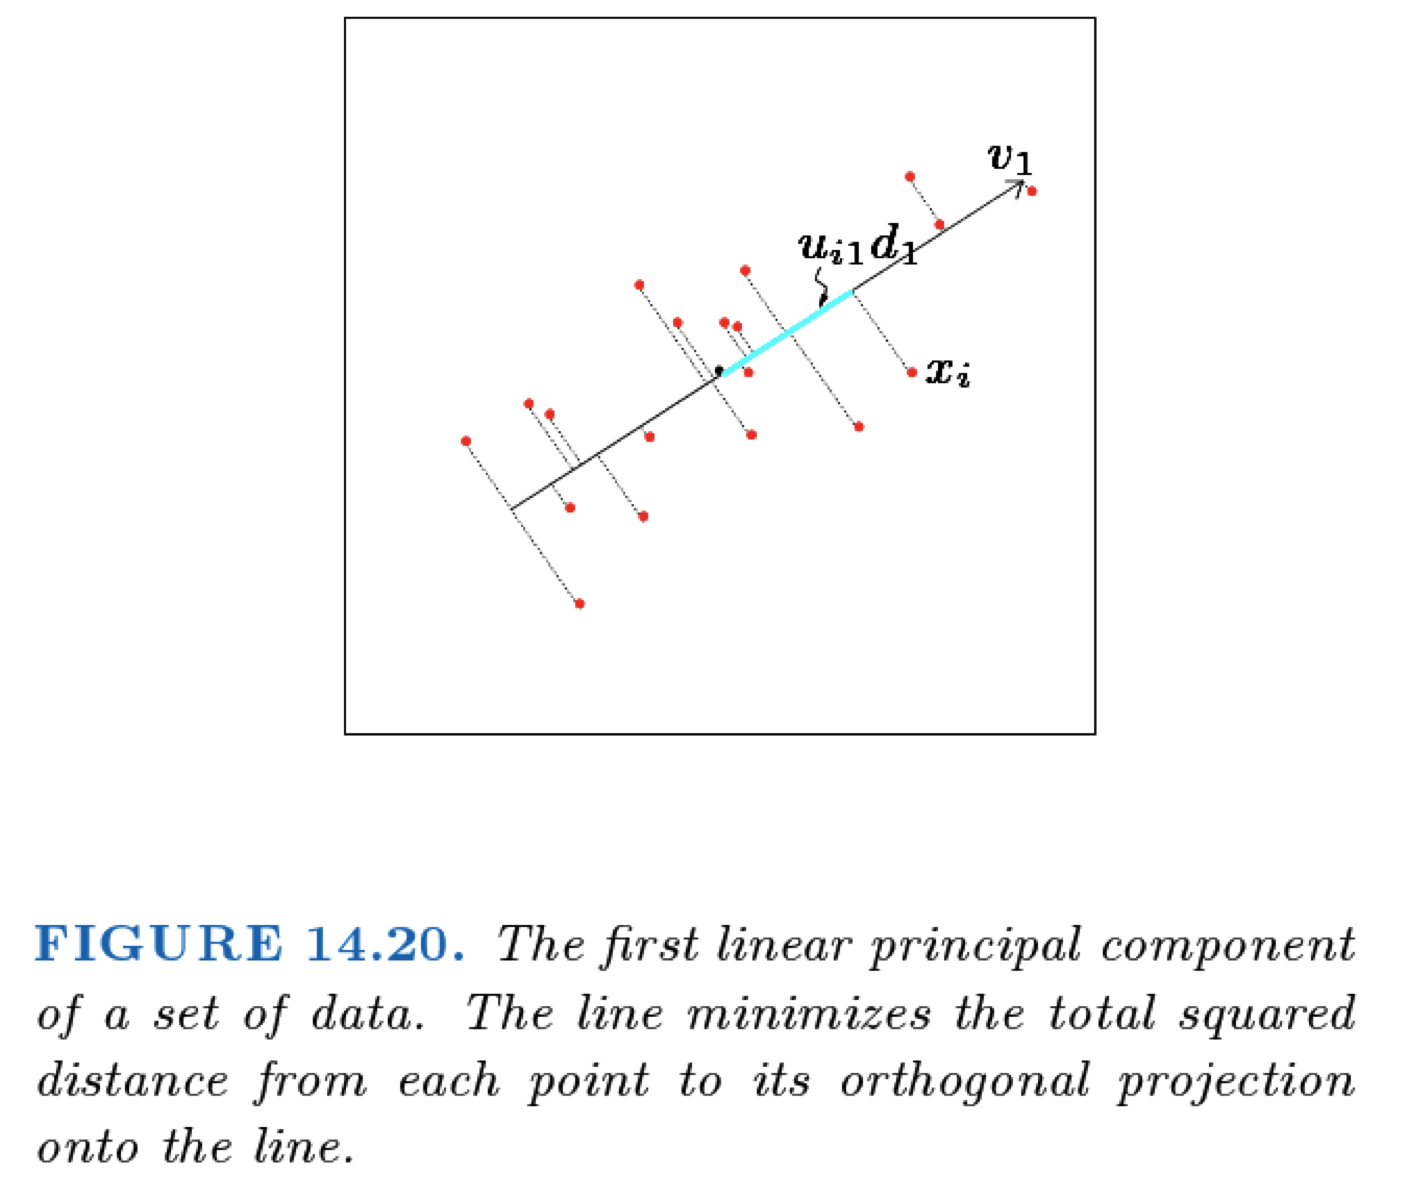
\includegraphics[width=1.0\textwidth]{TwoDimReduction.png}
\caption{\label{fig:2DimReduction} }
\end{figure}

As a simple example of dimensionality reduction, suppose you collect the feet length and width measurements for a group of people.  This yields a list of 2D feature vectors per person.  We would like to ``project this down'' to 1D in a manner that captures as much of the variability in the data ase possible.  In particular, if we can find the axis with greatest variance
as shown in Figure \ref{fig:2DimReduction}, the single coordinate of each data point along that axis could be a good choice for a reduced dimensionality representation of the data.

PCA attempts to capture the axes of variation by a sequence of projections of a dataset, mutually uncorrelated and ordered in variance. Being mutually uncorrelated we get a set of projections that do not contain duplication of data and assure we have the minimal set of projections containing the amount of data we need. By ordering the projections in variance we gain the ability to drop projections at the end of the list that are uninformative, that can perhaps be considered as noise, and by doing so reduce the dimentionality.\\

Given a set of $N$ points $x_i \in \mathbf{R}^p$, we suppose that they live on a linear manifold, rather than simply filing up $\mathbb{R}^p$ in an unstructured manner. The idea behind dimensionality reduction that PCA attempts to solve is to keep the best \emph{rank $q$ approximation} of the data for some $q<p$.  The model for representing the data is a non-parametric representation of an affine hyperplane of rank $q$:
$$f(\lambda)= \mu+\mathbf{V}_q \lambda$$
Where:
\begin{itemize}
\item $\mu$: a location vector in $\mathbf{R}^p$, can also be viewed as the ``centered'' origin of the data.
\item $\mathbf{V}_q \in \mathbf{R}^{p\times q}$, with $q$ orthogonal unit vectors as its columns.
\item $\lambda$: a vector of $q$ parameters.
\end{itemize}

\begin{figure}
\centering
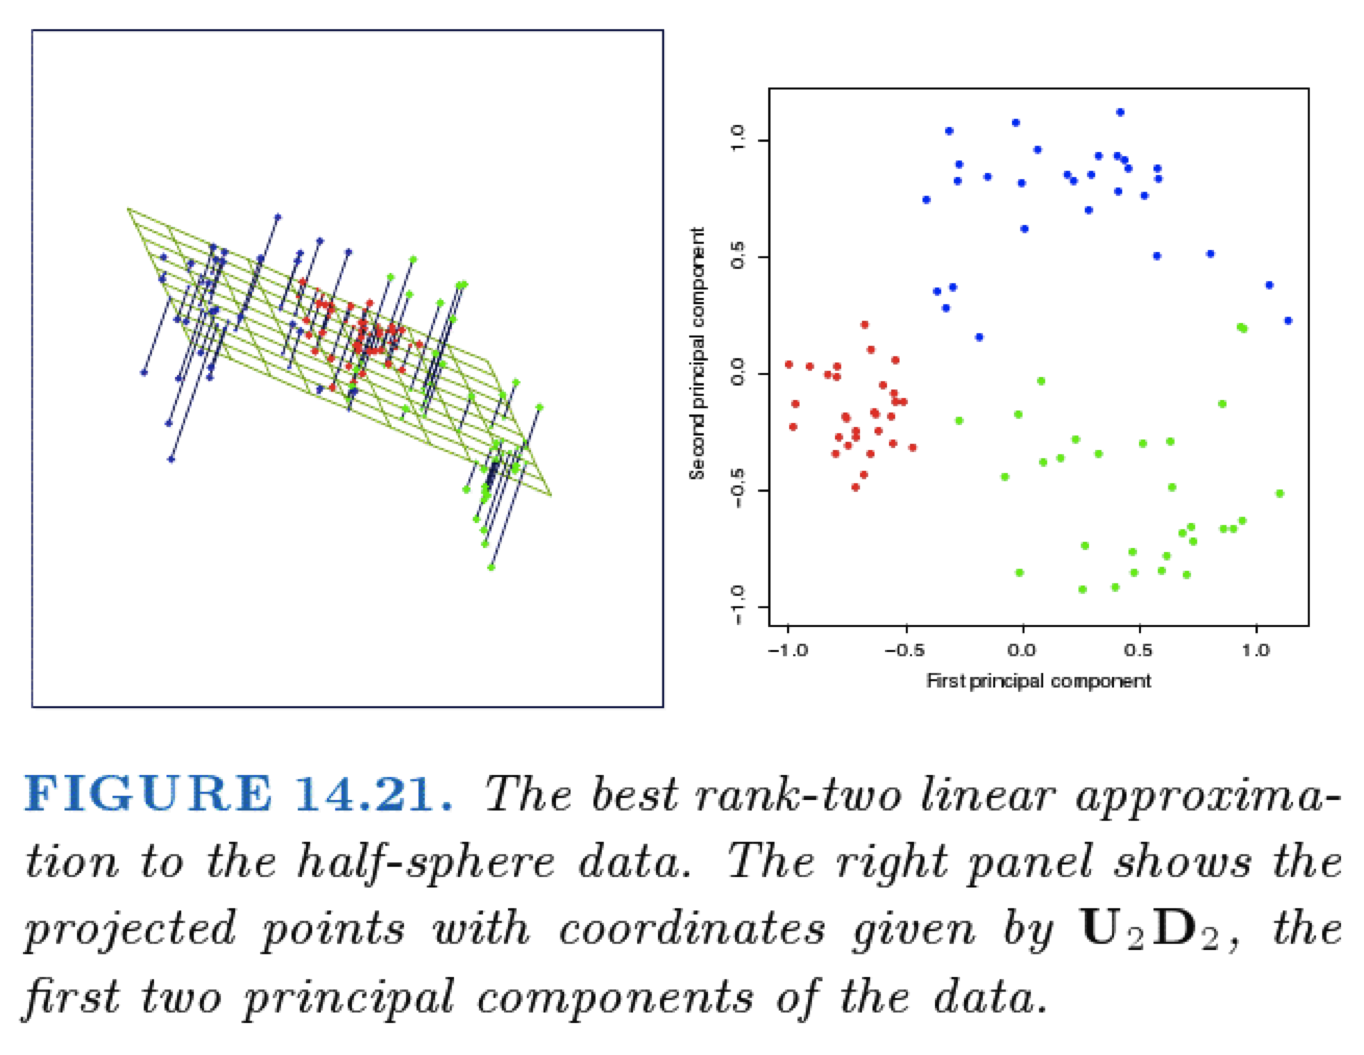
\includegraphics[width=1.0\textwidth]{ThreeDimReduction.png}
\caption{\label{fig:3DimReduction}}
\end{figure}

Figure \ref{fig:2DimReduction} is an example of a dimensionality reduction where $p=2$ and $q=1$. In Figure \ref{fig:3DimReduction} $p=3$ and $q=2$. 

We want to find the matrix $\mathbf{V}_q$ and vector $\lambda$ that generate the smallest reconstruction error. This is a least squares fitting problem:
$$\min_{\substack{
   \mu \\
   {\lambda_i} \\
   \mathbf{V}_q
  }} \sum_{i=1}^N \| x_i-\mu-\mathbf{V}_q\lambda_i \|^2$$
  
It is relatively straightforward to show that the optimal $\mu$ and $\lambda_i$s are given by:
\begin{itemize}
\item $\hat{\mu}=\bar{x}$: The new origin is the average of all the original data points, the center of the data.
\item $\hat{\lambda}_i=\mathbf{V}_q^\top(x_i-\bar{x})$: The projection after centering around the mean.
\end{itemize}

We are left with finding the optimal orthogonal matrix $\mathbf{V}_q$:
$$\min_{\mathbf{V}_q} \sum_{i=1}^N \| (x_i-\bar{x})-\mathbf{V}_q\mathbf{V}_q^\top(x_i-\bar{x})\|^2$$

For simplicity, assume we have a \textit{centered} set of data, i.e., $\bar{x}=0$, and we get:
$$\min_{\mathbf{V}_q} \sum_{i=1}^N \| x_i -\mathbf{V}_q\mathbf{V}_q^\top x_i \|^2$$
Where $\mathbf{V}_q\mathbf{V}_q^\top$ is a $p\times p$ projection matrix. Denote $\mathbf{M}_q=\mathbf{V}_q\mathbf{V}_q^\top$. $\mathbf{M}_q$ maps each $x_i$ onto its rank $q$ reconstruction, the orthogonal projection of $x_i$ onto the subspace spanned by the columns of $\mathbf{V}_q$. If $ p = q $, $\mathbf{V}_q\mathbf{V}_q^\top$  is an identity matrix.

We've already seen the machinery we need to solve this for $\mathbf{V}_q$: the SVD of $\mathbf{X}$, where $\mathbf{X}$ is formed by stacking the (centered) observations into the rows of an $N\times p$ matrix. The SVD of $\mathbf{X}$ is $\mathbf{U}\mathbf{D}\mathbf{V}^\top$, where $\mathbf{D}$ is a diagonal matrix with values $d_1, \ldots, d_p$ where: $d_1 \geq \ldots \geq d_p \geq 0$.
For each rank $q$ the solution to $\mathbf{V}_q$ above is given by the leading $q$ singular vectors in $\mathbf{V}$ (from the SVD). The columns of $\mathbf{UD}$ are the principal components of $\mathbf{X}$. The projection onto the sungular vectors gives us coordinates in a linear subspace, as shown in the right graph in Figure \ref{fig:3DimReduction}.

The sample covariance for $\mathbf{X}$, assuming it is centered, is:
$$\mathbf{S}=\frac{1}{N}\mathbf{X}^\top\mathbf{X}\in\mathbb{R}^{p\times p}$$
PCA computes the eigenvectors of $\mathbf{S}$ to reveal the orthogonal axes of variation in the data that capture the most variance, meaning the axes where the data spreads the most. PCA does this by throwing away small eigenvalues and their corresponding eigenvectors to leave the highest $q$ singular values.

\end{document}
